\pdfobjcompresslevel=1
\documentclass[compress,t]{beamer}

\newcommand{\niceurl}[1]{\mbox{\href{#1}{\textsl{#1}}}}

\usepackage{tikz}
%\usetikzlibrary{arrows,decorations.pathmorphing,backgrounds,placments,fit}
\usetikzlibrary{arrows.meta,decorations.pathmorphing,backgrounds,positioning,fit}

\usepackage{pdfpages}

% fonts p14; 18.2.3
% Futura font

% Cambridge, Copenhagen, JuanLesPins, Luebeck, Malmoe, Marburg,
% Montpellier, PaloAlto, Singapore

% colortheme beaver, dolphin

% Copyright 2004 by Till Tantau <tantau@users.sourceforge.net>.
%
% In principle, this file can be redistributed and/or modified under
% the terms of the GNU Public License, version 2.
%
% However, this file is supposed to be a template to be modified
% for your own needs. For this reason, if you use this file as a
% template and not specifically distribute it as part of a another
% package/program, I grant the extra permission to freely copy and
% modify this file as you see fit and even to delete this copyright
% notice. 

\mode<presentation> {
  \usetheme{Malmoe}
  \usecolortheme{beaver}
  \setbeamercovered{transparent}
  \setbeamertemplate{navigation symbols}{{\small\insertpagenumber}}
%{{\normalsize\insertframenumber}}
  \setbeamertemplate{footline}{%
    \leavevmode%
    \hbox{\begin{beamercolorbox}[wd=\paperwidth,ht=0.5ex,dp=1.125ex,leftskip=.3cm,rightskip=.3cm plus1fil]{title in head/foot}%
    \end{beamercolorbox}}%
    \vskip0pt%
  }
  \setbeamertemplate{headline}{% %split theme}
  \leavevmode%
    \begin{beamercolorbox}[wd=.7\paperwidth,ht=2.5ex,dp=1.125ex]{section in head/foot}%
      \insertsectionnavigationhorizontal{.3\paperwidth}{\hskip0pt plus1filll}{}%
  \end{beamercolorbox}%
  \begin{beamercolorbox}[wd=.3\paperwidth,ht=2.5ex,dp=1.125ex]{subsection in head/foot}%
    \insertsubsectionnavigationhorizontal{.7\paperwidth}{}{\hskip0pt plus1filll}%
  \end{beamercolorbox}%
  }
  %\setbeamersize{sidebar width right=2ex}
  %{\usebeamercolor{sidebar}}
  %\setbeamertemplate{sidebar canvas right}{f \insertframenumber}
  %\insertpagenumber
}

\usepackage[english]{babel}
\usepackage[latin1]{inputenc}
\usepackage{helvet}
\usepackage{xspace}
% Or whatever. Note that the encoding and the font should match. If T1
% does not look nice, try deleting the line with the fontenc.
%\usepackage[T1]{fontenc}
\usepackage[normalem]{ulem}
\usepackage{calc}
\usepackage{verbatim}
\usepackage{multirow}
\usepackage{dcolumn}
\usepackage{multimedia} 
%\usepackage{amsbsy}
\usepackage{amsmath}

\newcommand{\arxiv}[1]{\href{http://arxiv.org/abs/#1}{arXiv:#1}}
\newcommand{\etal}{\textit{et al.~}}
\newcommand{\snr}[1]{\mathbb{SN}(#1)}


\graphicspath{{figs-slides/}{figs-techreport/}}

\newcommand{\an}{\emph{Astrometry.net}\xspace}
\newcommand{\libkd}{\emph{libkd}\xspace}
\newcommand{\kdtree}{$kd$-tree}
\newcommand{\antoc}{Astrometry.net\xspace}
\newcommand{\eg}{\emph{eg}}

% holmes
\newcommand{\light}[1]{{\color{gray}#1}}

\newcommand{\paramvector}[1]{\boldsymbol{#1}}
\newcommand{\pointing}{\paramvector{\alpha}}
\newcommand{\fovpars}{\paramvector{\Omega}}
\newcommand{\orbitpars}{\paramvector{\omega}}
\newcommand{\hyperpars}{\paramvector{\theta}}
\newcommand{\position}{\paramvector{x}}
\newcommand{\velocity}{\paramvector{v}}
\newcommand{\uniform}{\mathrm{uniform}}
\newcommand{\tmin}{t_\mathrm{min}}
\newcommand{\tmax}{t_\mathrm{max}}
\newcommand{\pgood}{p_\mathrm{good}}
\newcommand{\pempirical}{p_\mathrm{emp}}
\newcommand{\pemp}{\pempirical}
\newcommand{\exif}{\mathrm{EXIF}}
\newcommand{\pexif}{p_\exif}
\newcommand{\texif}{t_\exif}
\newcommand{\pfg}{p_\mathrm{fg}}
\newcommand{\pbg}{p_\mathrm{bg}}

% commands to add more space in \itemize environments
\newcommand{\bitmorespace}{%
  \addtolength{\itemsep}{0.5ex}%
  %\addtolength{\parskip}{0.5ex}%
  %\addtolength{\parsep}{0.5ex}%
  %\addtolength{\topsep}{0.5ex}%
  \vspace{0.5ex}%
}
\newcommand{\morespace}{\addtolength{\itemsep}{1ex}}
\newcommand{\Morespace}{\addtolength{\itemsep}{1.5ex}}


\newcommand{\commentout}[1]{}


\usefonttheme[onlymath]{serif}
\usepackage{multimedia} 

\title{Markov Chain Monte Carlo}
\author{Dustin Lang}
\date{2019-09-17}

\begin{document}

\begin{frame}
  \titlepage
\end{frame}

%\section{Intro}

\begin{frame}{Markov Chain Monte Carlo for data analysis}
  \only<1>{%
    \begin{itemize}
    \item MCMC generates samples from a probability distribution function
    \item For data analysis: you have some \emph{measurements} $X$, with uncertainties
    \item have a \emph{model} for the thing you're measuring
    \item with unknown \emph{parameters} $\theta$
    \item the model is \emph{generative} -- predicts measurements given parameters
    \item MCMC can put constraints on the parameters given your measurements
    \end{itemize}
  }%
  \only<2>{%
    \begin{itemize}
    \item can think of it as: \emph{model} is a function mapping parameters to observables $t$: $m(\theta) \to t$
    \item and \emph{measurement process} gives probability of observing $X$ given $t$: $P(X | t)$
    \item (eg, maybe $P(X | t)$ is a Gaussian with zero mean and standard deviation $\sigma$)
    \item Then, can chain $P(X | t) = P(X | m(\theta))$
    \item Usually, we fold $m$ and $P$ together to write $P(X | \theta)$
    \end{itemize}
  }%
  \only<3>{%
    \begin{itemize}
    \item $P(X | \theta)$ (the ``likelihood'') is not what you want!
    \item You want $P(\theta | X)$ -- the ``posterior'' -- constraints on / measurements of the parameters
    \item Good thing you're Bayesian!
    \item ``posterior'' $P(\theta | X) = \frac{P(X | \theta) P(\theta)}{P(X)}$
    \item $P(\theta)$ is the ``prior''
    \item $P(X)$ is the ``evidence'', and in this setting is constant (ignored)
    \end{itemize}
  }%
  \only<4>{%
    \begin{itemize}
    \item We'll use MCMC to draw samples from the \emph{posterior} probability distribution
    \item $P(\theta | X) = P(X | \theta) P(\theta)$
    \item The samples are a set of $\theta$ values drawn from your parameter constraints distribution
    \end{itemize}
  }%
\end{frame}

\begin{frame}{What's in a name}
  \begin{itemize}
  \item \emph{Monte Carlo} -- a famous casino in Monaco -- alluding to the use of \emph{randomness} in the algorithm
  \item \emph{Chain} -- a list (here, a list of samples / steps $\theta_1$, $\theta_2$, $\theta_3$)
  \item \emph{Markov Chain} -- a list of ``steps'' where the decision to step from $\theta_{i}$ to $\theta_{i+1}$
    depends only on the value of $\theta_i$
  \end{itemize}

  \begin{itemize}
  \item \emph{Metropolis--Hastings} -- first authors of 1953 and 1970 papers (resp) with the simplest, most commonly taught algorithm
  \end{itemize}
\end{frame}

\begin{frame}{Using MCMC}
  \begin{itemize}
  \item ``Just write down the probability distributions''
  \item hah, the ``model to predictions'' part, $m(\theta) \to t$, can be \emph{very} difficult
  \item eg, in cosmology, the software \emph{CAMB} does this, in 25,000 lines of FORTRAN
  \item writing down the \emph{likelihood} might take some work too!
  \end{itemize}
\end{frame}

\begin{frame}{MCMC: the idea}
  \begin{itemize}
  \item move a ``particle'' or ``walker'' around in the parameter space $\theta$, based on the value of the
    probability function \\ (for us: the posterior probability $P(\theta | X)$)
  \item choose new parameters according to a \emph{proposal distribution}
    -- often Gaussian: $\theta_{new} = \theta + \mathcal{N}(0, \Sigma)$
  \item compute probability at new $\theta_{new}$ and decide whether to move (``jump'') to new parameters
  \item \emph{always} keep improvements, \emph{sometimes} keep decreases
  \item in the long run, the set of walker positions $\{ \theta_1, \theta_2, \theta_3, ... \}$ are your samples
  \end{itemize}
\end{frame}

\begin{frame}[fragile]{Finally, M--H MCMC code}
\begin{verbatim}
fun MCMC(prob_function, sample_proposal, params, Nsteps):
    chain = []
    prob = prob_function(params)
    for i in 1 to Nsteps:
        # sample from proposal distribution
        params_new = sample_proposal(params)
        prob_new = prob_function(params_new)
        # accept?
        if ((prob_new > prob) OR
            (prob_new / prob) > uniform_random()):
            params = params_new
            prob = prob_new
        chain.append(params)
    return chain
\end{verbatim}
\end{frame}

\begin{frame}{Demo}
  Credit: Dan Foreman--Mackey
  \niceurl{https://speakerdeck.com/dfm/data-analysis-with-mcmc}
\end{frame}


% Use example from DanFM:
%  wget https://speakerd.s3.amazonaws.com/presentations/1cbbeda07de1013062221231381d8c65/vanderbilt.pdf
% pdfjam vanderbilt.pdf 1-1,31-54 --papersize '{5.04in,3.78in}' -o vanderbilt-sub.pdf
{
\setbeamercolor{background canvas}{bg=}
\includepdf[pages=2-25,fitpaper=true]{vanderbilt-sub.pdf}
}

\begin{frame}{MCMC: summary}
  Things MCMC can do for you
  \begin{itemize}
  \item produce constraints on model parameters, including covariances
  \item include (but ignore) \emph{nuisance parameters} in your data analysis
  \end{itemize}
  
  Things MCMC doesn't do for you
  \begin{itemize}
  \item tell you if it has converged!
  \item tell you if your model is good
  \item (easily) allow comparisons between models
  \item handle multi-modal distributions (try \emph{nested sampling})
  \item Dan Foreman--Mackey has good notes on \href{https://github.com/LSSTC-DSFP/LSSTC-DSFP-Sessions/blob/master/Session10/Day2/AdvancedSampling.ipynb}{\alert{advanced sampling methods}}
  \end{itemize}
\end{frame}

\end{document}
